\begin{figure}[htbp]

\centering
\begin{subfigure}[t]{0.49\textwidth}
\captionsetup{labelformat=empty}

\caption{\textbf{AAPL}}
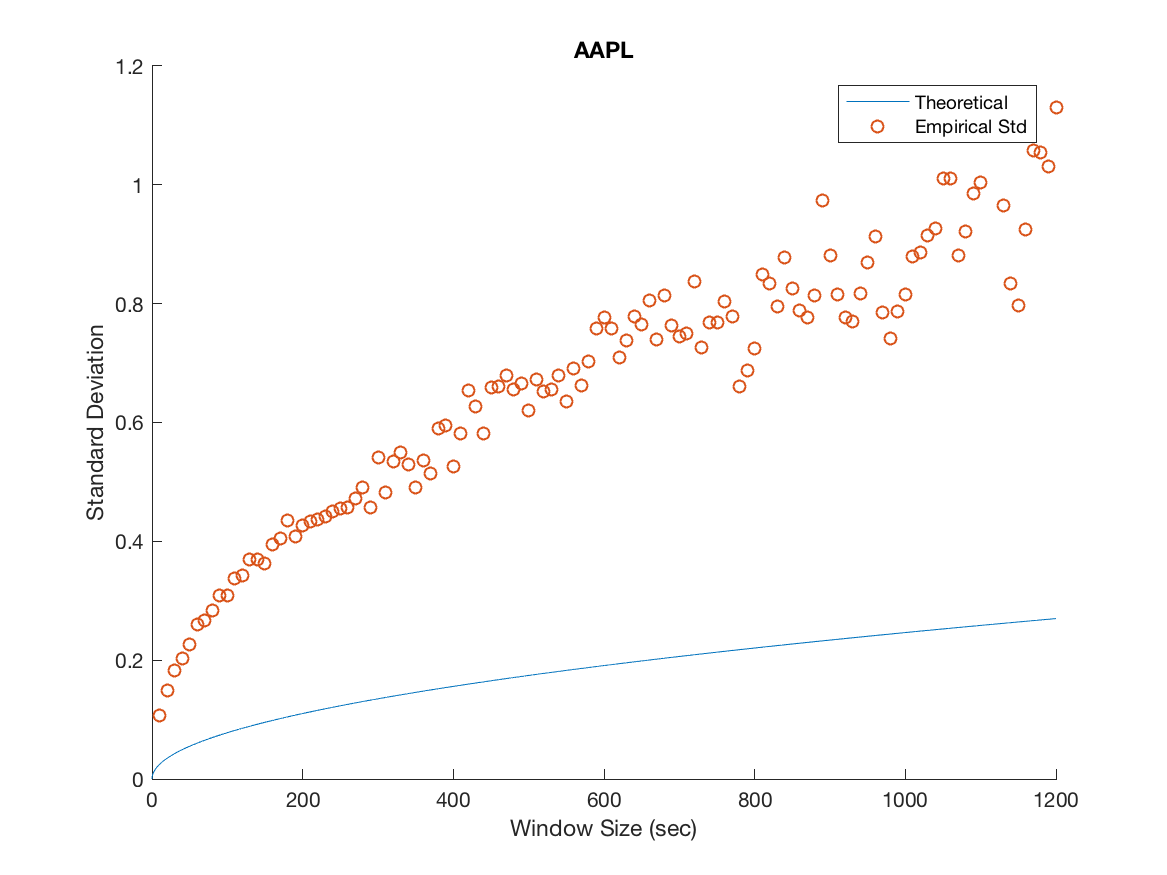
\includegraphics[width=\textwidth, trim = 0 0 0 30, clip]{CHPDO_Fit/AAPL_Plot_CHPDO_21600.png}

\end{subfigure}
\begin{subfigure}[t]{0.49\textwidth}
\captionsetup{labelformat=empty}

\caption{\textbf{AMZN}}
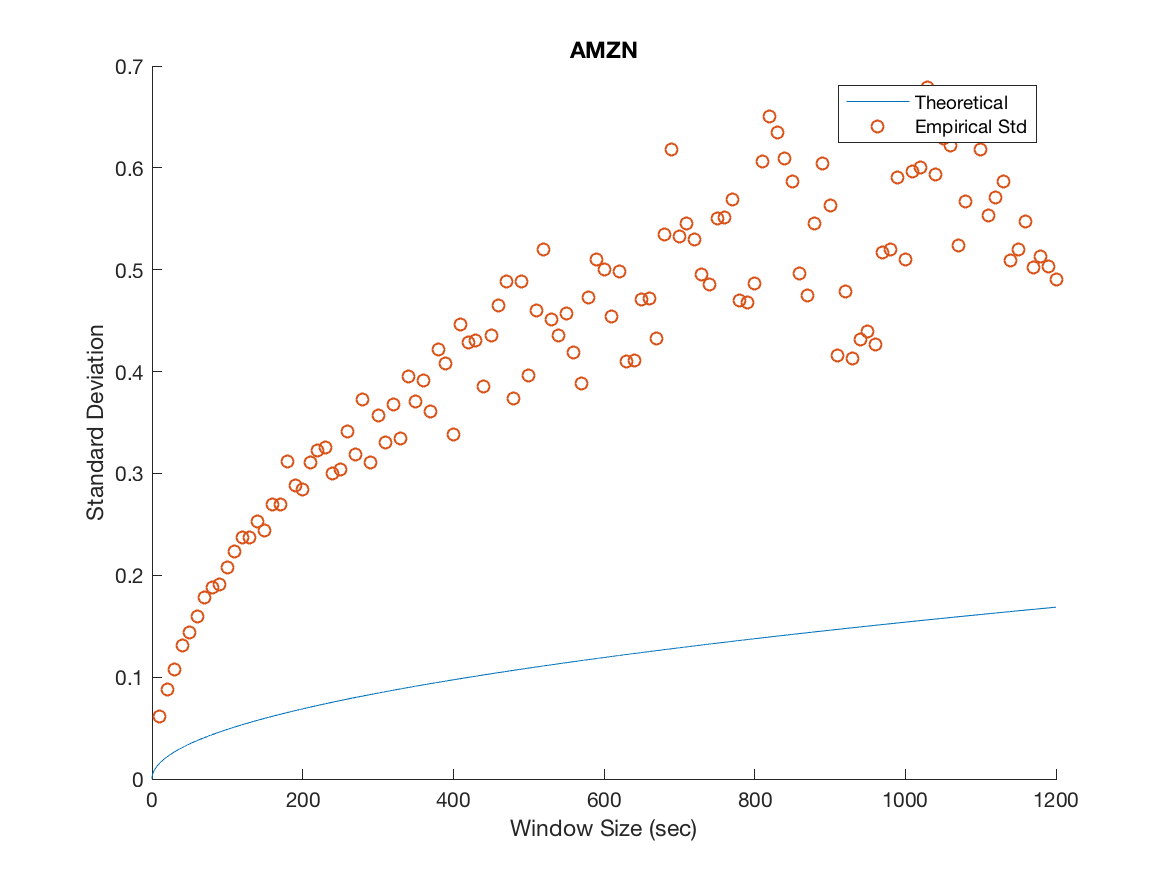
\includegraphics[width=\textwidth, trim = 0 0 0 30, clip]{CHPDO_Fit/AMZN_Plot_CHPDO_21600.png}
\end{subfigure}

\vspace{3mm}

\begin{subfigure}[t]{0.49\textwidth}
\captionsetup{labelformat=empty}

\caption{\textbf{GOOG}}
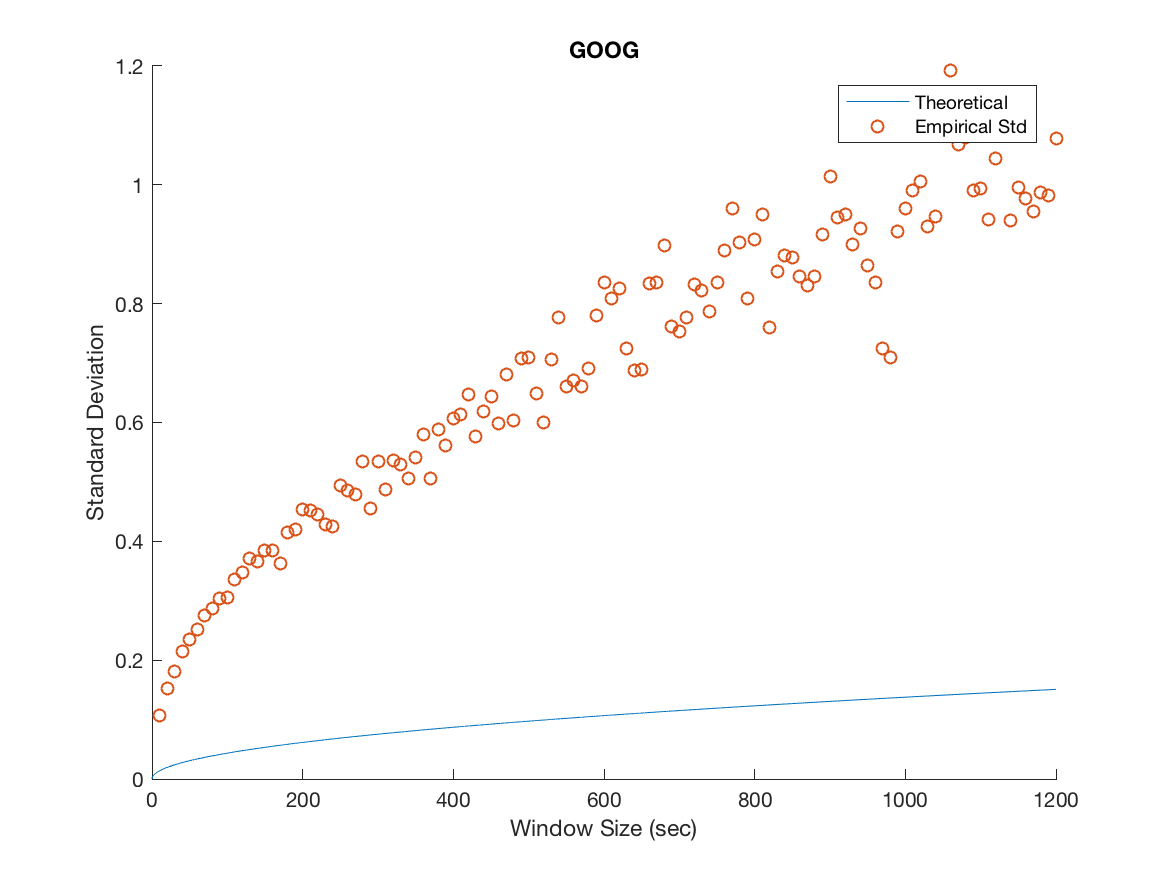
\includegraphics[width=\textwidth, trim = 0 0 0 30, clip]{CHPDO_Fit/GOOG_Plot_CHPDO_21600.png}

\end{subfigure}
\begin{subfigure}[t]{0.49\textwidth}
\captionsetup{labelformat=empty}

\caption{\textbf{INTC}}
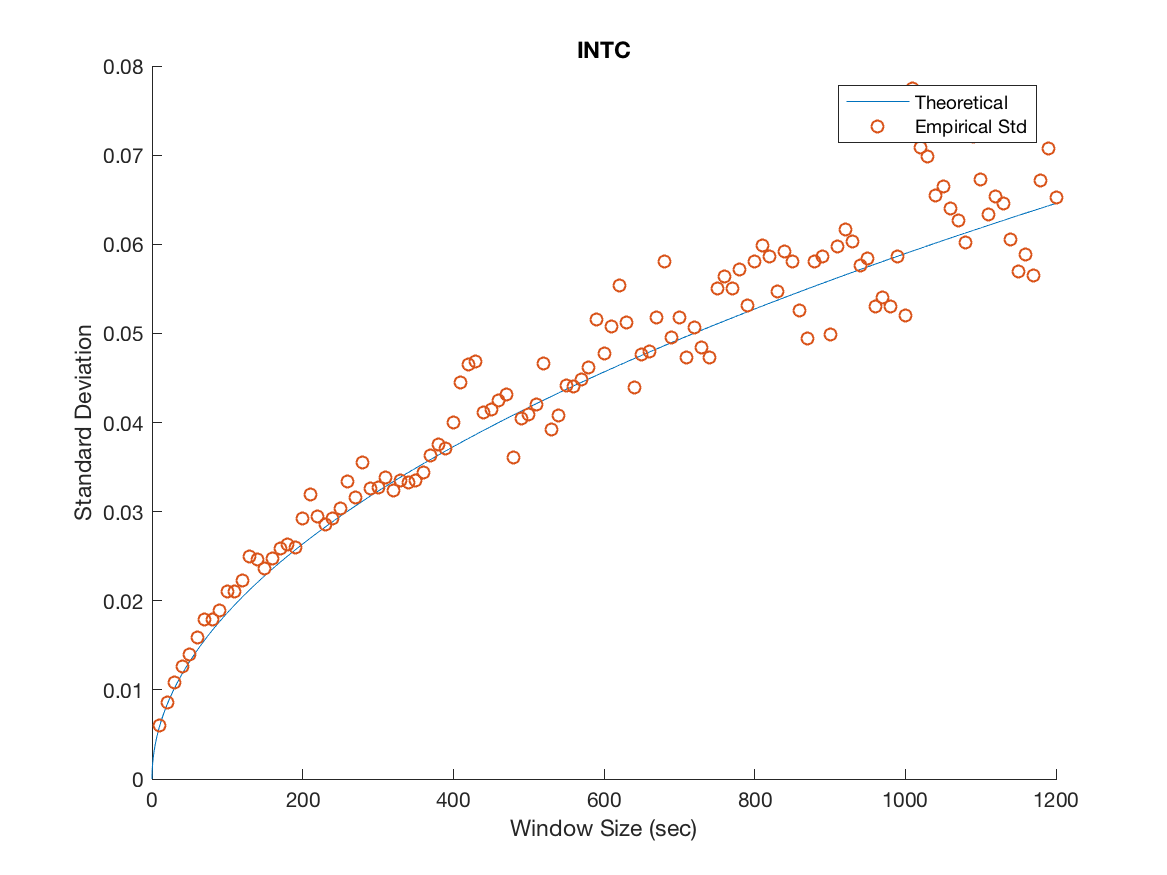
\includegraphics[width=\textwidth, trim = 0 0 0 30, clip]{CHPDO_Fit/INTC_Plot_CHPDO_21600.png}
\end{subfigure}

\vspace{3mm}

\begin{subfigure}[t]{0.49\textwidth}
\captionsetup{labelformat=empty}

\caption{MSFT}
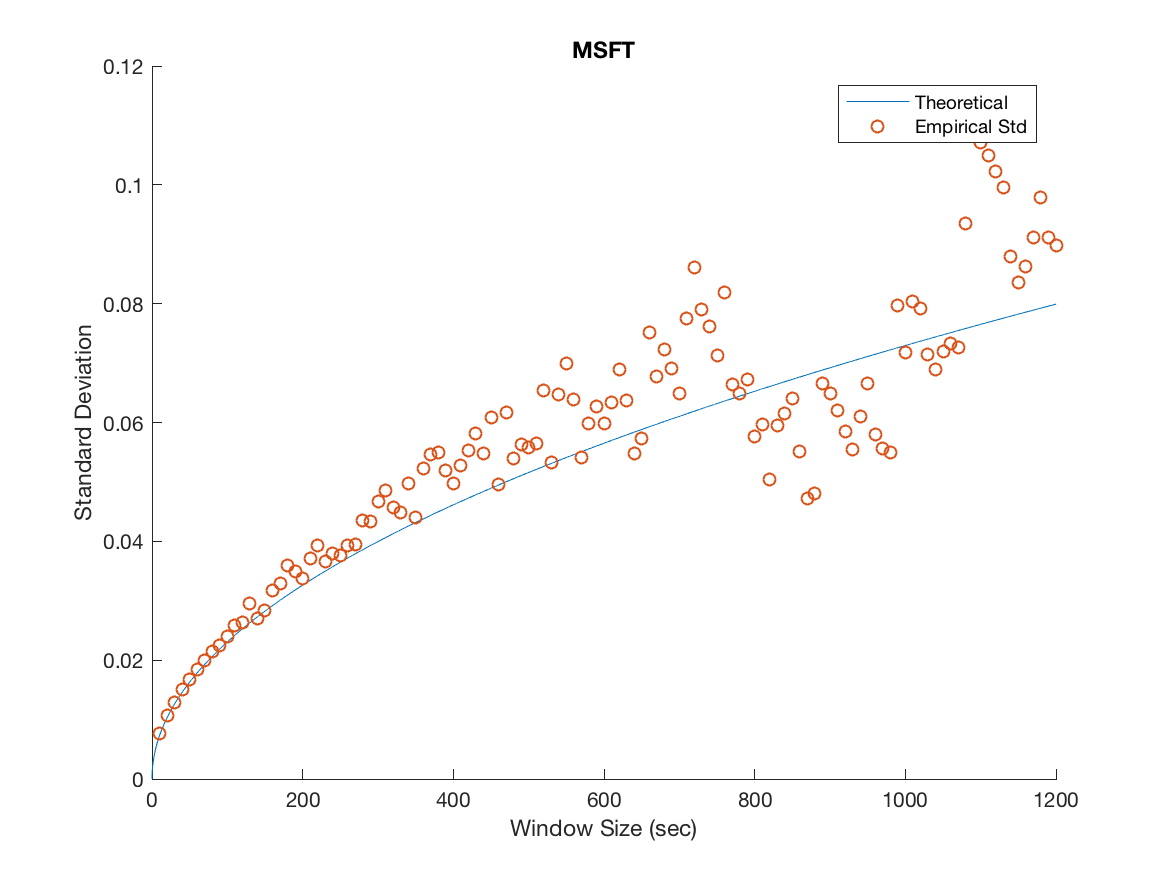
\includegraphics[width=\textwidth, trim = 0 0 0 30, clip]{CHPDO_Fit/MSFT_Plot_CHPDO_21600.png}
\end{subfigure}

\caption{\label{fig:chpdofit} Each figure compares the empirical standard deviation for a fixed window size to the theoretical standard deviation. We have plotted an empirical standard deviation for all $n$ from 10 seconds to 20 minutes in step sizes of 10 seconds. Each empirical standard deviation corresponds to a single point in the scatter plot and the plotted curve corresponds to the predicted theoretical value.}


\end{figure}